\documentclass[a4paper, 10pt, fleqn]{article}

\usepackage{layout}

\author{Pascal Häfliger, Fabian Niederberger, Marc Nussbaumer, Daniel Winz}
\title{Projektauftrag "Vier Gewinnt"}

\begin{document}
\maketitle
\tableofcontents
\newpage

\section{Einleitung}
Geschätzte Studierende

In der zweiten Hälfte des Semesters bearbeiten Sie in einer kleinen Gruppe 
ein kleineres Softwareprojekt. Mit diesem Projekt sind die folgenden Ziele 
verbunden:
\begin{itemize}
    \item Sie wenden im Unterricht gelernte Konzepte der Sprache Java in 
        einem grösseren Kontext an.
    \item Sie wiederholen wesentliche Elemente der Programmiersprache Java.
    \item Sie implementieren eine Softwarelösung im Team.
    \item Sie können Kontextdiagramme lesen und interpretieren.
    \item Sie können Komponentendiagramme lesen und interpretieren.
    \item Sie können Sequenzdiagramme lesen und interpretieren.
    \item Sie können Zustandsdiagramme lesen und interpretieren.
    \item Sie können Sourcecode mit Hilfe von Klassendiagrammen dokumentieren.
    \item Sie können in einem grösseren Programm die Übersicht wahren.
\end{itemize}
Das gesamte Projekt ist als Lernprojekt zu verstehen, bei dem Sie Schritt 
für Schritt Kenntnisse erwerben und anwenden. \\
Die Dozierenden und Assistierende begleiten Sie während des Projekts und 
ermöglichen Ihnen, wesentliche Erfahrungen zu reflektieren. Zur Unterstützung 
dieses Prozesses erstellen Sie jede Woche für die Dozierenden einen kurzen 
Projekt-Statusrapport mit folgendem Inhalt:
\begin{itemize}
    \item Welche Arbeiten wurden in der letzten Woche ausgeführt. Was hat gut 
        geklappt, wo hatten oder haben Sie Probleme?
    \item Welche Tätigkeiten sind für die nächste Woche vorgesehen?
    \item Welche Knackpunkte (Herausforderungen oder Risiken) bestehen noch? 
        Was gedenken Sie dagegen zu unternehmen?
\end{itemize}
Eine Vorlage für diesen Projekt-Statusrapport [2] finden Sie im ILIAS.
\\\\
Viel Erfolg sowie spannende und wertvolle Projekterfahrungen wünschen Ihnen
\\\\
Ihr Dozierendenteam

\section{Glossar}

\section{Anforderungen}
Der Projektauftrag wurde handschriftlich abgegeben.

>>>FIXME Anforderungen ableiten

\subsection{Regeln Vier Gewinnt}
“Das Spiel wird auf einem senkrecht stehenden hohlen Spielbrett gespielt, in 
das die Spieler abwechselnd ihre Spielsteine fallen lassen. Das Spielbrett 
besteht normalerweise aus sieben Kolonnen (senkrecht) und sechs Reihen 
(waagerecht). Jeder Spieler besitzt mind. 21 gleichfarbige Spielsteine. Wenn 
ein Spieler einen Spielstein in eine Spalte fallen lässt, besetzt dieser den 
untersten freien Platz der Spalte. Gewinner ist der Spieler, der es als erster 
schafft, vier oder mehr seiner Spielsteine waagerecht, senkrecht oder diagonal 
in eine Linie zu bringen. Das Spiel endet unentschieden, wenn das Spielbrett 
komplett gefüllt ist, ohne dass ein Spieler eine Viererlinie gebildet hat.”

\subsection{Stories}
\begin{figure}[h!]
    \center
    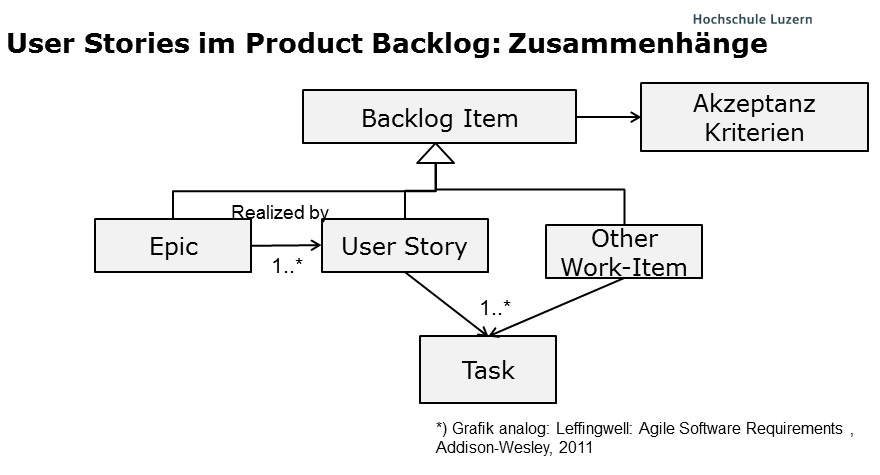
\includegraphics[width=\textwidth]{fig/stories.png}
\end{figure}
Aus den Anforderungen werden Backlog Items (nach Scrum) generiert. Die Epics 
bilden in diesem Projekt 1:1 die Stories aus den Anforderungen ab. Epics (E) 
bestehen aus Stories (S) und Stories aus Tasks (T). Tasks sind die kleinste 
Einheit und von einer Person in einem Sprint bearbeitbar. Auf Ebene Epic/Story 
gibt es noch Other Work-Items (O). Mit diesen werden alle Tasks abgearbeitet, 
welche nicht einer Story oder einem Epic zugeordnet werden können.
\begin{itemize}
    \item \#O Architektur
    \begin{itemize}
        \item 
        \begin{itemize}
            \item \#T Schnittstelle zwischen Komponenten definieren
            \item \#T Pro Komponente wesentliche Klassen identifizieren
            \item \#T Interaktion dieser Komponenten
        \end{itemize}
    \end{itemize}
    \item \#E1 Vier Gewinnt gegen den Computer spielen
    \begin{itemize}
        \item \#S1 - Als Spieler möchte ich, dass die Spielregeln von Vier 
            Gewinnt eingehalten werden.
        \begin{itemize}
            \item \#T Züge validieren (Regeln von Vier Gewinnt)
            \item \#T Gewinnbedingungen ermitteln (Ende des Spiels)
            \item \#T Spielablauf (Steuerungslogik) festlegen (Control)
            \item \#T Modell aufbauen
            \item \#T Schnittstellen Model, Control definieren
        \end{itemize}
        \item \#S2 - Als Spieler möchte ich das Spiel am Bildschirm sehen und 
            mit der Maus spielen können.
        \begin{itemize}
            \item \#T Schnittstellen View definieren
            \item \#T View mit Swing implementieren
        \end{itemize}
        \item \#S3 - Als Spieler möchte ich gegen einen einfachen 
            Computergegner spielen können.
        \begin{itemize}
            \item \#T RandomComputerOpponent implementieren
        \end{itemize}
        \item \#S8 - Als Spieler möchte ich gegen einen schlauen 
            Computergegner spielen können. 
        \begin{itemize}
            \item \#T AwareComputerOpponent implementieren 
        \end{itemize}
    \end{itemize}
    \item \#E2 Im Netz nach menschlichen Gegenspielern suchen und einen 
        Gegenspieler auswählen. Der Gegenspieler darf den ersten Spielstein 
        setzen.
    \begin{itemize}
        \item \#S4 - Als Spieler möchte ich aus allen im Netzwerk verfügbaren 
            Gegenspielern auswählen können. 
        \begin{itemize}
            \item \#T Schittstelle “available Opponents” definieren
            \item \#T Broadcast implementieren
            \item \#T View (Auswahl Opponent) implementieren
        \end{itemize}
        \item \#S5 - Als Spieler möchte ich gegen einen menschlichen 
            Gegenspieler spielen können.
        \begin{itemize}
            \item \#T Netzwerkprotokoll definieren
            \item \#T Moves über Netzwerk in Control implementieren
        \end{itemize}
        \item \#S6 - Als Gegenspieler möchte ich eine Herausforderung zum 
            Spiel annehmen können.
        \begin{itemize}
            \item \#T View (Frage + Buttons YES/NO) implementieren
            \item \#T OpponentResponse über Netzwerk in Control implementieren
        \end{itemize}
    \end{itemize}
    \item \#E3 Wenn ich gegen den Computer spiele, möchte ich das Spiel 
        unterbrechen, speichern und später mit dem gleichen Spielstand 
        weiterspielen können.
    \begin{itemize}
        \item \#S7 - Als Spieler möchte ich, wenn ich gegen den Computer 
            spiele, das Spiel unterbrechen, speichern und später mit dem 
            gleichen Spielstand weiterspielen können.
        \begin{itemize}
            \item \#T Schnittstelle View-Control erweitern
            \item \#T Model Serializeable machen
            \item \#T Button in View implementieren
            \item \#T Control Save/Load Command implementieren
        \end{itemize}
    \end{itemize}
\end{itemize}

\subsection{Environment}
\begin{itemize}
    \item Für das Spiel über Netzwerk muss Traffic über UDP erlaubt sein, 
        insbesondere müssen UDP-Broadcasts erlaubt sein.
    \begin{itemize}
        \item Weil UDP-Broadcast im HSLU-Netz nicht erlaubt sind, wird ein 
            Wifi Access-Point im F-Stock/Bunker zur Verfügung gestellt. Die 
            Angaben dazu lauten:
        \begin{itemize}
            \item SSID: 
            \item Passwort: 
        \end{itemize}
    \end{itemize}
    \item Java muss in (mindestens) der Version 1.7 installiert sein.
\end{itemize}

\section{Systemspezifikation}
Die folgende Kapiteleinteilung lehnt sich an die “Vier Arten von Sichten” 
aus Gernot Starke: \href{http://books.google.ch/books?id=CaqQAgAAQBAJ&pg=PA80}
{"Effektive Softwarearchitekturen: Ein praktischer Leitfaden" (16.01.2014), 
Seite 80, Kapitel 4.4.2, Bild 4.31 an.}

\subsection{Kontextabgrenzung}

\subsubsection{Lokales Spiel}
\begin{figure}[h!]
    \center
    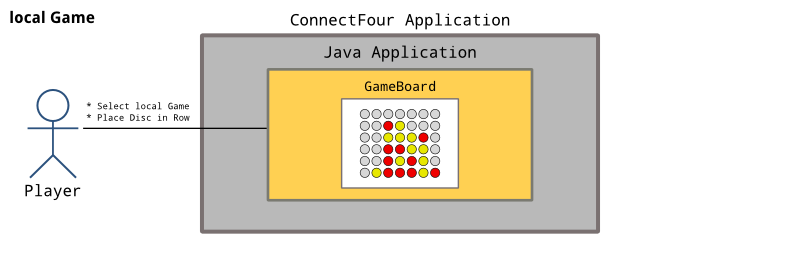
\includegraphics[width=\textwidth]{fig/local-game.png}
\end{figure}

\subsubsection{Netzwerk-Spiel}
\begin{figure}[h!]
    \center
    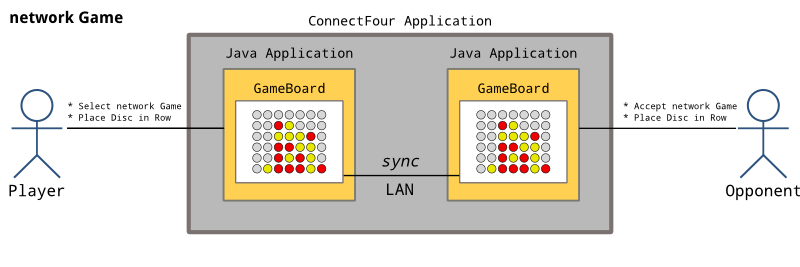
\includegraphics[width=\textwidth]{fig/network-game.png}
\end{figure}

\subsection{Bausteinesichten}

\subsubsection{Komponentendiagramm}
\begin{figure}[h!]
    \center
    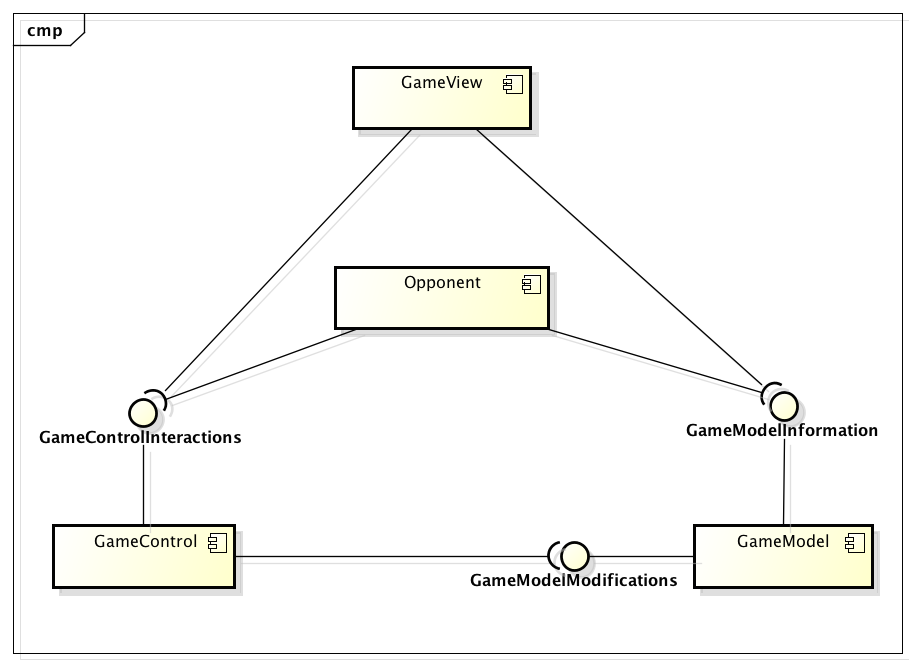
\includegraphics[width=\textwidth]{fig/components.png}
\end{figure}
Dieses Diagramm zeigt die Komponenten der Applikation. Opponent kann ein 
lokaler Computer-Opponent oder ein entfernter Netzwerk-Opponent sein.

\subsubsection*{GameControlInteractions}
Über diese Schnittstellen können Opponent und GameView Befehle an die 
GameControl absetzen (z.B. Neues Spiel, Gegner ausgewählt, etc.).

\subsubsection*{GameModelInformation}
Interessierte Klassen werden über diese Schnittstelle über Änderungen am 
GameModel informiert.

\subsubsection*{GameModelModifications}
Über diese Schnittstelle kann die GameControl Änderungen am GameModel 
vornehmen.

\subsubsection{Klassendiagramme}
>>>FIXME Inhalt des Kapitels: Mindestens für jede Komponente ein Klassendiagram.

\subsubsection{MVC}
Für die Anwendung wird das Model-View-Controller Entwurfsmuster (MVC) 
verwendet. (Siehe: 
\url{http://de.wikipedia.org/wiki/Model_View_Controller})\\\\
Nachfolgendes Sequenzdiagramm beschreibt das Einfügen eines Spielsteins nach 
dem Klick im GUI:
\begin{figure}[h!]
    \center
    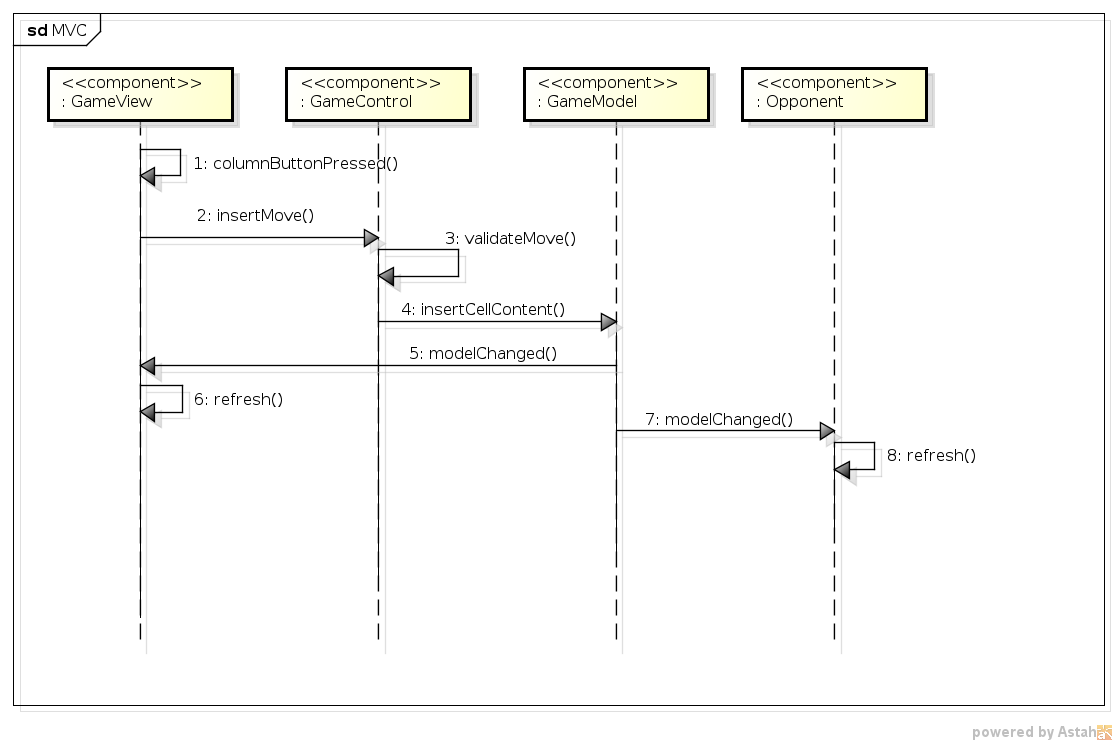
\includegraphics[width=\textwidth]{fig/seq.png}
\end{figure}

\subsubsection{GameModel}
GameModel enthält den aktuellen Zustand des Spiels. Also zum Beispiel die 
aktuellen Spieler, ihre Steine auf dem Spielbrett usw. Das Model notifiziert 
Listeners falls es sich geändert hat (z.B. mit dem Observer-Pattern 
\url{http://en.wikipedia.org/wiki/Observer_pattern}). Listeners können sich 
mit der Methode \verb?void addModelListener(final GameModelListener listener)? 
beim Model für Notifications registrieren. Listeners sind zum Beispiel die 
View oder ein Opponent.

\subsubsection{GameView}
GameView wird durch das Model notifiziert, falls sich etwas am Model geändert 
hat und stellt anschliessend das Model grafisch dar. Also zum Beispiel die 
aktuellen Spieler, ihre Steine auf dem Spielbrett usw. Ausserdem leitet die 
View Eingaben des Benutzers (Disc in Kolonne eingefügt, Neues Spiel etc.) an 
das Control weiter.

\subsubsection{GameControl}
Das GameControl empfängt Input (Commands von Opponent oder View), entscheidet 
ob die Commands gültig sind und darf als einziges das Model ändern.

\subsubsection{Opponent}
Opponent wird vom Model notifiziert, wenn das Model geändert hat und darf 
Befehle an das Control senden. Der Opponent besitzt damit viel Ähnlichkeit 
mit der View. Entsprechend können hier gemeinsame Schnittstellen definiert 
werden.

\subsection{Laufzeitsichten}

\subsubsection{Zustandsautomat}
\begin{figure}[h!]
    \center
    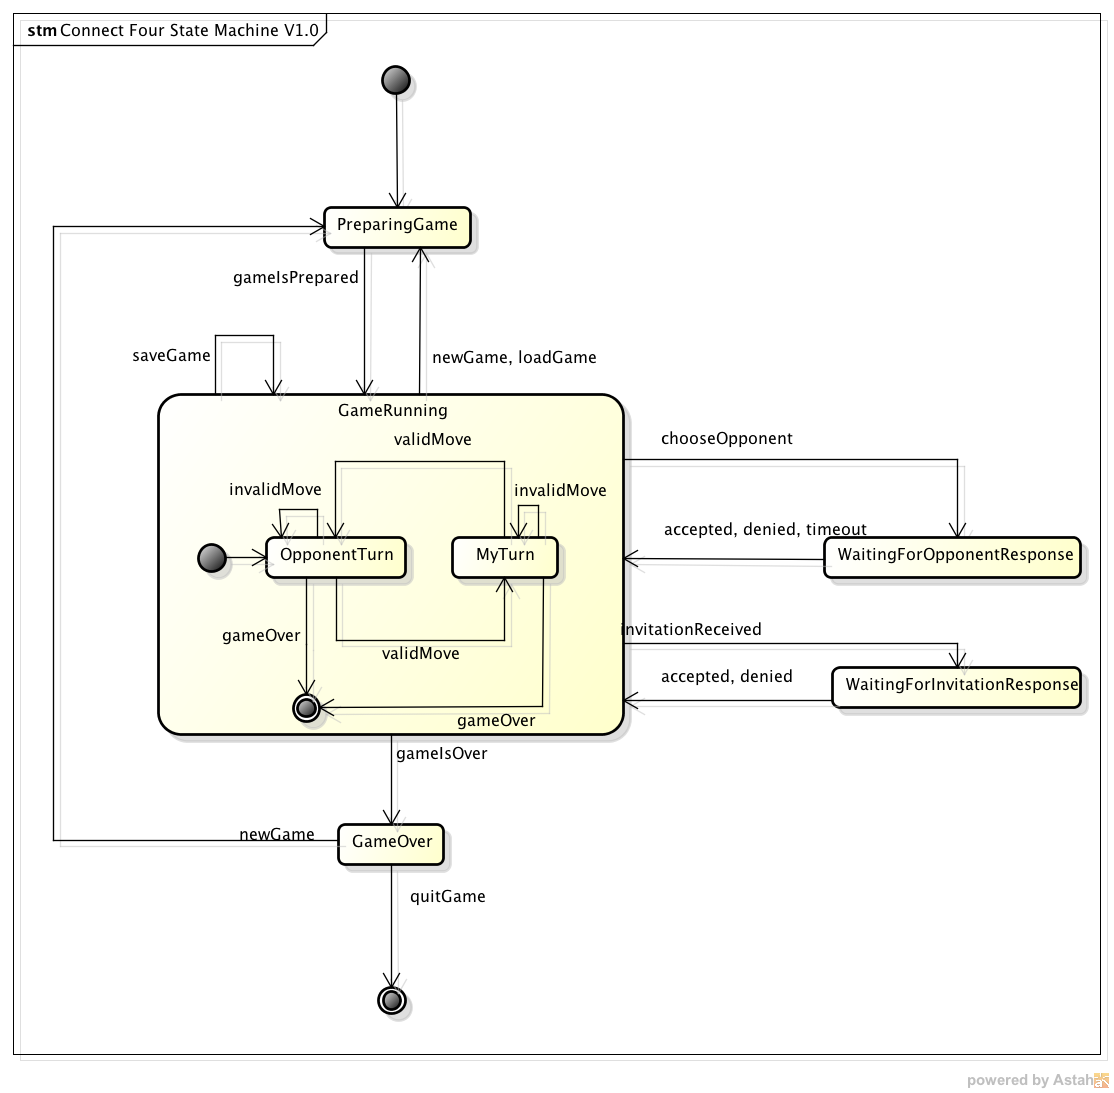
\includegraphics[width=\textwidth]{fig/state.png}
\end{figure}
In rundenbasierten Spielen lässt sich häufig ein Zustandsautomat einsetzen. 
Dies kann durch zwei verschachtelte Zustandsautomaten realisiert werden. Der 
Äussere kümmert sich um Vorbereitung und Nachbearbeitung des Spiels, während 
sich der Innere um den Ablauf während dem Spiel kümmert.

\subsubsection*{PreparingGame}
Das Spielfeld wird aufgebaut und die Teilnehmenden werden initialisiert. 
Der/die erste Spieler/in ist ein Mensch, der/die zweite wird zunächst auf 
einen Computergegner gesetzt, damit sofort mit dem Spiel begonnen werden kann. 
Nach dem Aufbau des Spielfelds geht der Zustand per gameIsPrepared unmittelbar 
in den Zustand GameRunning (bzw. konkret direkt in OpponentTurn) über.

\subsubsection*{GameRunning}
>>>FIXME Zustand beschreiben

\subsubsection*{MyTurn}
>>>FIXME Zustand beschreiben

\subsubsection*{OpponentTurn}
>>>FIXME Zustand beschreiben

\subsubsection*{WaitingForOpponentResponse}
>>>FIXME Zustand beschreiben

\subsubsection*{WaitingForInvitationResponse}
Falls über das Netzwerk eine Anfrage zur Teilnahme an einem anderen Spiel 
eintrifft, geht der Zustand von “GameRunning” (bzw. konkret einem seiner 
Unter-Zustände \verb?OpponentTurn? oder \verb?MyTurn?) per 
\verb?invitationReceived? über in \verb?WaitingForInvitationResponse?. Dort 
wird ausgewählt, ob die Einladung angenommen werden soll oder nicht. 
Unabhängig von dieser Entscheidung geht der Zustand danach per 
\verb?accepted?, \verb?denied? wieder in \verb?GameRunning? über.

\subsubsection*{GameOver}
>>>FIXME Zustand beschreiben

\subsection{Verteilungssicht}
>>>FIXME Inhalt dieses Kapitels: 
\begin{itemize}
    \item Wie läuft die Applikation im Betrieb?
    \item Auf welchen Rechner läuft die Applikation?
\end{itemize}

\subsection{Datensicht}
>>>FIXME Inhalt dieses Kapitels: 
\begin{itemize}
    \item Wie sieht die Applikation aus Datensicht aus?
    \item Was für Daten werden vor der Applikation verwaltet, geteilt, gespeichert?
\end{itemize}

\subsection{Netzwerkprotokoll}
>>>FIXME Netzwerkprotokoll beschreiben
\begin{itemize}
    \item Wie sieht die Kommunikation über das Netzwerk aus?
    \item Gibt es ein Protokoll?
\end{itemize}

\section{Erweiterungsmöglichkeiten}
Eigene Erweiterungen dokumentieren \\
Folgende Erweiterungen sind für das Projekt denkbar:
\begin{itemize}
    \item Variable Grösse des Spielfelds
    \item Computergegner gegeinander antreten lassen
    \item Der Verlauf einer Partie kann aufgezeichnet und wieder abgespielt werden
\end{itemize}




\end{document}
